% Header
\renewcommand\evenpagerightmark{{\scshape\small Chapter 4}}
\renewcommand\oddpageleftmark{{\scshape\small Amplification processes in gaseous detectors}}

\renewcommand{\bibname}{References}

\hyphenation{}

\chapter[Physics of Resistive plate chambers]%
{Physics of Resistive plate chambers}
\label{chapt:4}

A \acf{RPC} is a gaseous detector used in high-energy physics experiments as described in Chapter~\ref{chapt:3}. It has been developed in 1981 by Santonico and Cardarelli~\cite{SANTONICO81}, under the name of \textit{Resistive Plate Counter}, as an alternative to the local-discharge spark counters proposed in 1978 by Pestov and Fedotovich~\cite{PESTOV78,FEDOTOVICH82}. Working with spark chambers implied using high-pressure gas and high mechanical precision which the RPC simplified by formerly using a gas mixture of argon and butane flowed at atmospheric pressure and a constant and uniform electric field propagated in between two parallel electrode plates. Moreover, a significant increase in rate capability was introduced by the use of electrode plate material with high bulk resistivity, preventing the discharge from growing throughout the whole gas gap. Indeed, the effect of using resistive electrodes is that the constant electric field is locally canceled out by the development of the discharge, limiting its growth.
	
	Through its development history, different operating modes~\cite{CROTTY93,CROTTY94,CARDARELLI96} and new detector designs~\cite{ZEBALLOS96MRPC,WILLIAMS98,CZYRKOWSKI98} have been discovered, leading to further improvement of the rate capability of such a detector. The low developing costs and easily achievable large detection areas offered by RPCs, as well as the wide range of possible designs, made them a natural choice to as muon chambers and/or trigger detectors in multipurpose experiments such as CMS~\cite{MUONTDR} or ATLAS~\cite{ATLASTDR}, time-of-flight detectors in ALICE~\cite{ALICETDR}, calorimeter with CALICE~\cite{CALICE2016} or even detectors for volcanic muography with ToMuVol~\cite{TOMUVOL2011}. 

\section{Principle}
\label{chapt4:sec:principle}

	RPCs are ionisation detectors composed of two parallel resistive plate electrodes in between which a constant electric field is set. The space in between the electrodes, referred to as \textit{gap}, is filled with a dense gas that is used to generate primary ionization into the gas volume. The free charge carriers (electrons and cations) created by the ionization of the gas molecules are then accelerated towards the electrodes by the electric field, as shown in Figure~\ref{fig:RPC_principle}~\cite{LIPPMANN2003}. RPCs being passive detectors, a current on pick-up copper read-out placed outside of the gas volume is induced by the charge accumulation during the growth of the avalanche resulting from the acceleration of the charge carriers. As a consequence, the time resolution of the detector is substantially increased as the output signal is generated while the electrons are still in movement. The advantage of a constant electric field, over multi-wire proportional chambers, is that the electrons are being fully accelerated from the moment charge carriers are freed and feel the full strength of the electric field that doesn't depend on the distance to the readout and that the output signal doesn't need for the electrons to be physically collected.
	
	\begin{figure}[H]
		\centering
		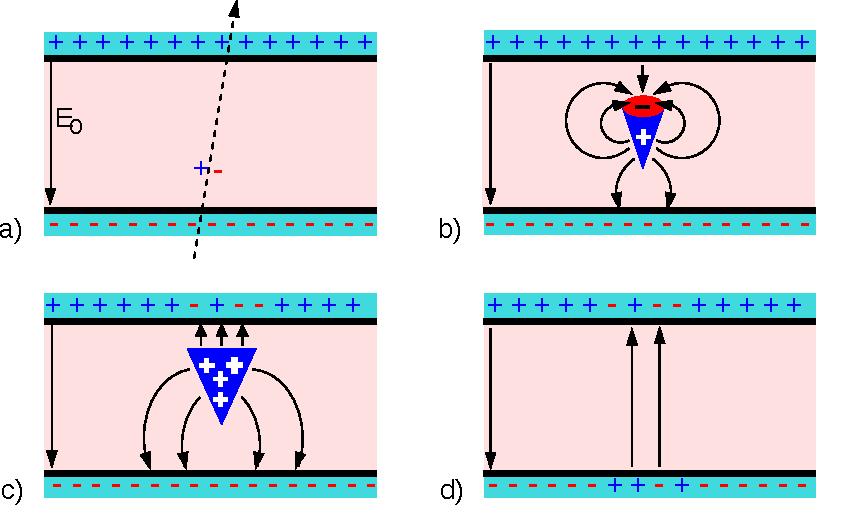
\includegraphics[width = \plotwidth]{fig/chapt4/RPC_principle.pdf}\\
		\caption{\label{fig:RPC_principle} Different phases of the avalanche development in the RPC gas volume subjected to a constant electric field $E_0$. a) An avalanche is initiated by the primary ionisation caused by the passage of a charged particle through the gas volume. b) Due to its growing size, the avalanche starts to locally influence the electric field. c) The electrons, lighter than the cations reach the anode first. d) The ions reach the cathode. While the charges have not recombined, the electric field in the small region around the avalanche stays affected and locally blinds the detector.}
	\end{figure}
	
	After an avalanche developed in the gas, a time long compared to the development of a discharge is needed to recombine the charge carriers in the electrode material due to their resistivity. This property has the advantage of affecting the local electric field and avoiding sparks in the detector but, on the other hand, the rate capability is intrinsically limited by the time constant $\tau_{RPC}$ of the detector. Using a quasi-static approximation of Maxwell’s equations for weakly conducting media, it can be shown that the time constant $\tau_{RPC}$ necessary to the charge recombination at the interface in between the electrode and the gas volume is given by the Formula~\ref{for:tau}~\cite{RIEGLER2002}.
	
	\begin{equation}
		\label{for:tau}
		\tau_{RPC} = \frac{\epsilon_{electrode}+\epsilon_{gas}}{\sigma_{electrode}+\sigma_{gas}}
	\end{equation}
	
	A gas can be assimilated to vacuum, leading to $\epsilon_{gas} = \epsilon_0$ and $\sigma_{gas} = 0$, and the electrodes permittivity and conductivity can be written as $\epsilon_{electrode} = \epsilon_r\epsilon_0$ and $\sigma_{electrode} = 1/\rho_{electrode}$, showing the strong dependence of the time constant to the electrodes resistivity in Formula~\ref{for:taurho}.
	
	\begin{equation}
		\label{for:taurho}
		\tau_{RPC} = (\epsilon_r + 1)\epsilon_0\times\rho_{electrode}
	\end{equation}
	
	Very few materials with a low enough resistivity exist in nature. The resistivity targeted to build RPCs ranges from $10^9$ to $10^{12}$ \si{\ohm\cdot cm}. The most common RPC electrode materials are displayed in Table~\ref{tab:tau}. When the doped glass and ceramics can offer short time constants of the order of \SI{1}{ms}, the developing cost of such materials is quite high due to the very low demand. Thus, \acf{HPL} is often the choice for high rate experiments using very large RPC detection areas. Other experiments working at cosmic muon fluxes can safely operate with ordinary float glass.
	
	\begin{table}[H]
		\centering
		\begin{tabular}{|l|c|c|c|}
		\hline
		Material & $\rho_{electrode}$ (\si{\ohm\cdot cm}) & $\epsilon_r$ & $\tau_{RPC}$ (\si{ms})\\
		\hline
		Float glass & $10^{12}$ & $\sim$7 & $\sim$700\\
		\acl{HPL} & $10^{10}$ to $10^{12}$ & $\sim$6 & $\sim$6 to 600\\
		Doped glass (LR S) & $10^{9}$ to $10^{11}$ & $\sim$10 & $\sim$1 to 100\\
		Doped ceramics (SiN/SiC) & $10^{9}$ & $\sim$8.5 & $\sim$1\\
		Doped ceramics (Ferrite) & $10^{8}$ to $10^{12}$ & $\sim$20 & $\sim$0.2 to 2000\\
		\hline
		\end{tabular}
		\caption{\label{tab:tau} Properties of the most used electrode materials for RPCs.}
	\end{table}

\section{Rate capability and time resolution of Resistive Plate Chambers}
\label{chapt4:sec:RateCapa}

	The electrode material plays a key role in the maximum intrinsic rate capability of RPCs. R\&D is continuously being done to develop at always cheaper costs material with lower resistivity. Nevertheless, the amount of charge released, i.e. the size of the discharge, if reduced leads to a smaller blind area in the detector, increasing the rate capability of the detector. On the other hand, the drift velocity of electrons in the gas volume being quite stable with the applied electric field, the design of a detector and the associated read-out and pulse-processing electronics will be a major component of the time resolution of RPCs. Moreover, the sensitivity of the electronics will also help increasing the rate capability by lowering the gain the gas volume needs to be operated at, increasingly lowering the gas volume in which the signals will develop.
	
	\subsection{Operation modes}
	\label{chapt4:ssec:operation}
	
	Being a gaseous detector using an accelerating electric field to amplify the signal of primary charge carriers, the RPC can be operated into different modes as the electric field intensity varies. Each mode offers different performances for such a detector, and it will be showed that the operating mode corresponding to the lowest electric field possible is best suited for high rate detectors working in collider experiments.
	
	RPCs where developed early 1980s. At that time it was using an operating mode now referred to as \textit{streamer mode}. Streamers are large discharges that develop in between the 2 electrodes enough to locally discharge the electrodes. If the electric field inside of the gas volume is strong enough, with electrons being fast compared to ions, a large and dense cloud of positive ions will develop nearby the anode and extend toward the cathode while the electrons are being collected, eventually leading to a streamer discharge due to the increase of field seen at the cathode. The field is then strong enough so that electrons are pulled out of the cathode. Electrodes, though they are a unique volume of resistive material, can be assimilated to capacitors. At the moment an electric field is applied in between their outer surfaces, the charge carriers inside of the volume will start moving leading to a situation where there is no voltage across the electrodes and a higher density of negative charges, i.e. electrons, on the inner surface of the cathode. Finally, when a streamer discharge occurs, these electrons are partially released in the gas volume contributing to increase the discharge strength until the formation of a conductive plasma, the streamer. This can be understood through Figure~\ref{fig:ElecCharge}~\cite{CROTTY93}. Streamer signals are very convenient in terms of read-out as no further amplification is required with output pulses amplitudes of the order of a few tens to few hundreds of \si{mV} as can be seen on Figure~\ref{fig:ModeSignal}.
	
	\begin{figure}[H]
		\begin{subfigure}{0.5\linewidth}
			\centering
			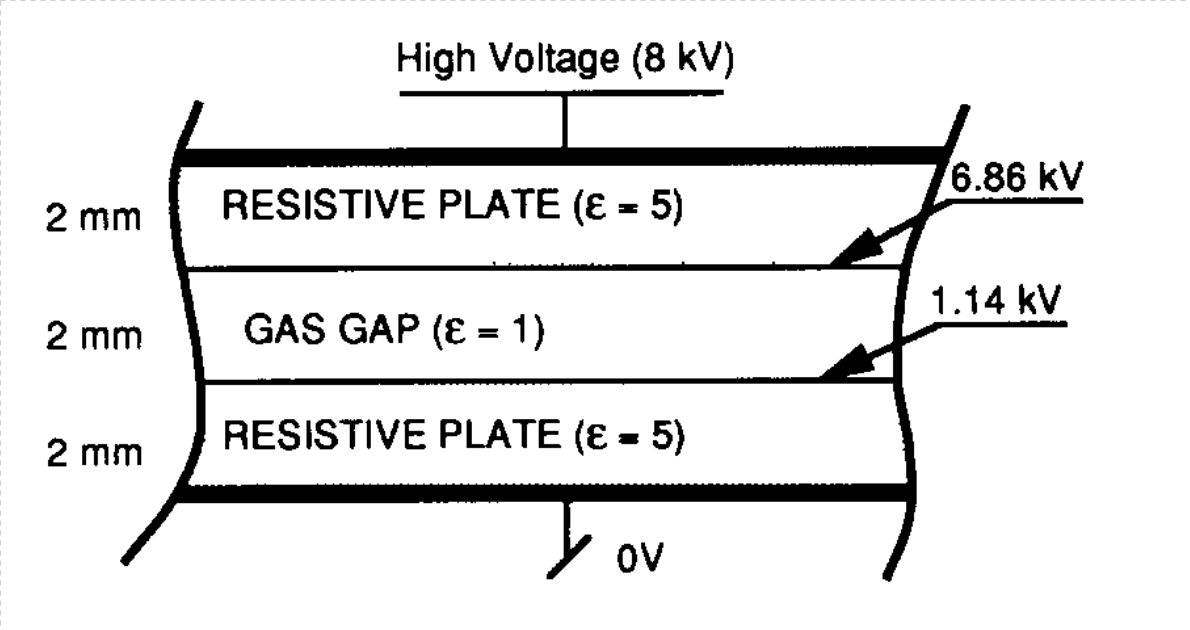
\includegraphics[width = 0.5\plotwidth]{fig/chapt4/RPC_Charging_1.png}
			\caption{\label{fig:ElecCharge:A}}
		\end{subfigure}
		\begin{subfigure}{0.5\linewidth}
			\centering
			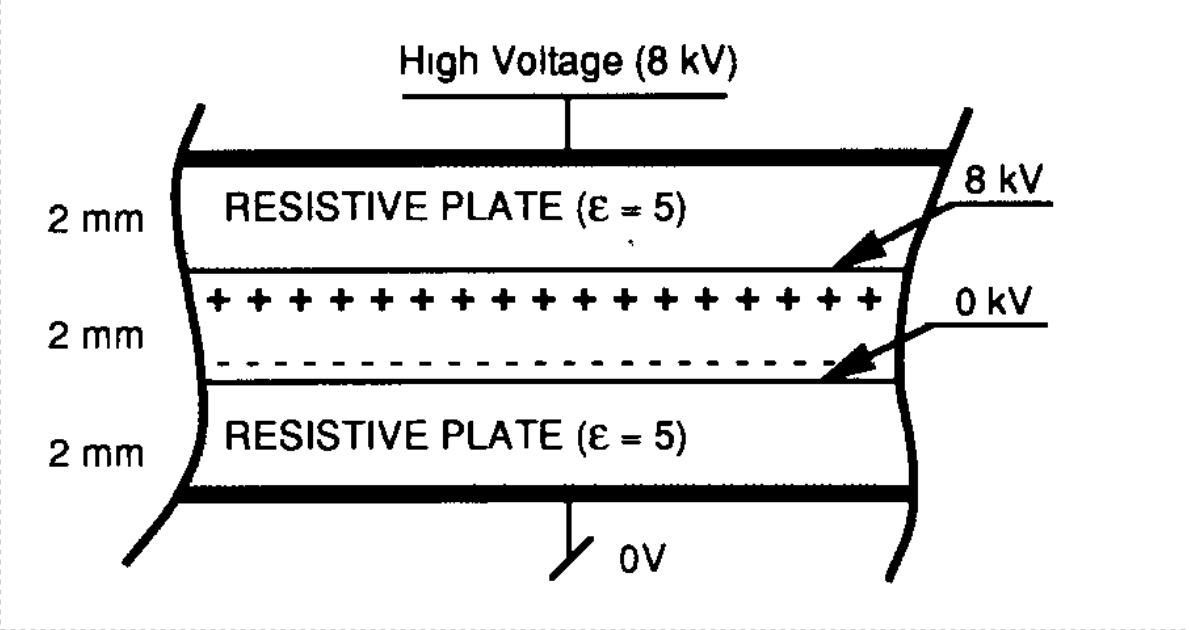
\includegraphics[width = 0.5\plotwidth]{fig/chapt4/RPC_Charging_2.png}\\
			\caption{\label{fig:ElecCharge:B}}
		\end{subfigure}
		\begin{subfigure}{\linewidth}
			\centering
			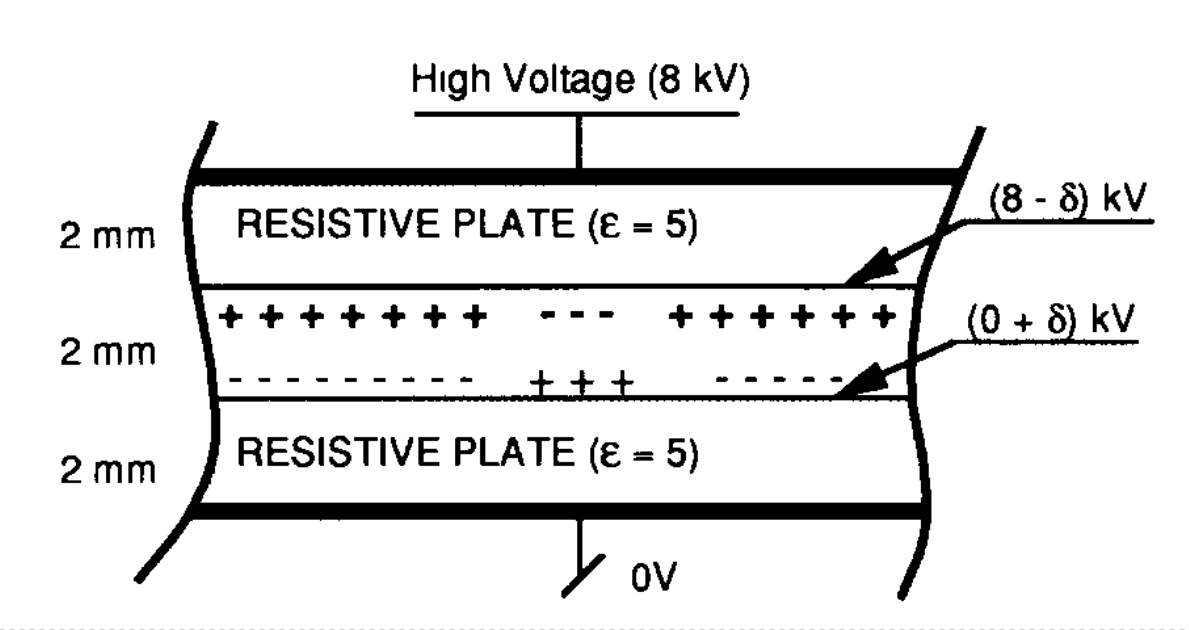
\includegraphics[width = 0.5\plotwidth]{fig/chapt4/RPC_Charging_3.png}
			\caption{\label{fig:ElecCharge:C}}
		\end{subfigure}
		\caption{\label{fig:ElecCharge} Movement of the charge carriers in an RPC. Figure~\ref{fig:ElecCharge:A}: Voltage across an RPC whose electrode have a relative permittivity of 5 at the moment the tension s applied. Figure~\ref{fig:ElecCharge:B}: After the charge carriers moved, the electrodes are charged and there is no voltage drop over the electrodes anymore. The full potential is applied on the gas gap only. Figure~\ref{fig:ElecCharge:C}: The streamer discharge initiated by a charged particle transports electrons and cations towards the anode and cathode respectively.}
	\end{figure}
	
	\begin{figure}[H]
		\begin{subfigure}{0.5\linewidth}
			\centering
			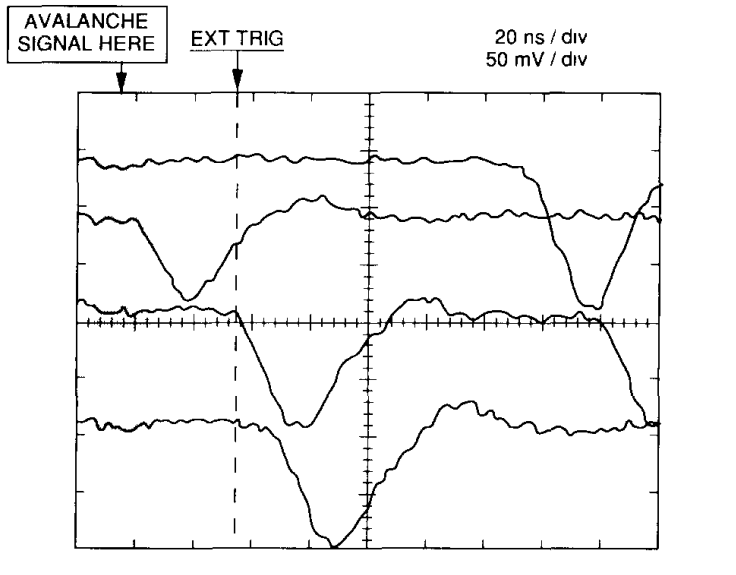
\includegraphics[width = 0.5\plotwidth]{fig/chapt4/RPC_Streamer_Mode.png}
			\caption{\label{fig:ModeSignal:A}}
		\end{subfigure}
		\begin{subfigure}{0.5\linewidth}
			\centering
			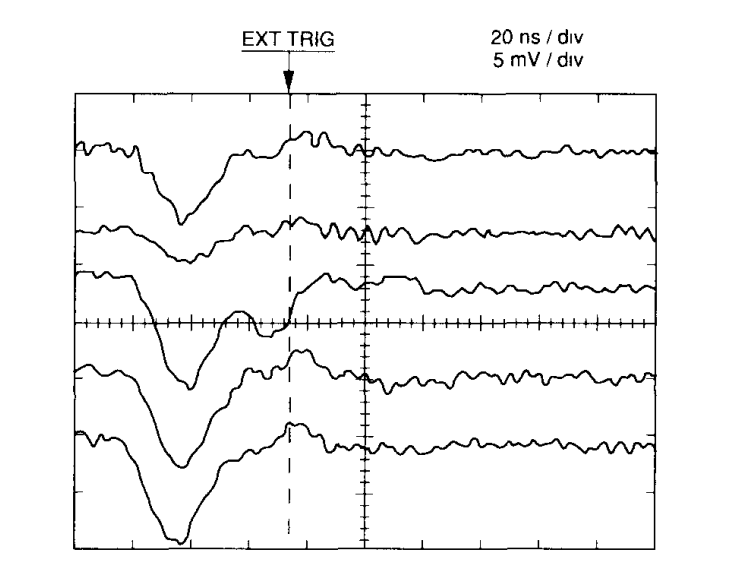
\includegraphics[width = 0.5\plotwidth]{fig/chapt4/RPC_Avalanche_Mode.png}\\
			\caption{\label{fig:ModeSignal:B}}
		\end{subfigure}
		\caption{\label{fig:ModeSignal} Typical oscilloscope pulses in streamer mode (Figure~\ref{fig:ModeSignal:A}) and avalanche mode(Figure~\ref{fig:ModeSignal:B}). In the case of streamer mode, the very small avalanche signal is visible.}
	\end{figure}
	
	When the electric field is reduced though, the electronic gain is small until the electrons get close enough to the anode and the positive ion cloud is much smaller. The electric field cannot rise to the point a field emission of electrons on the cathode is possible. The resulting signal is weak, of the order of a few \si{mv} as shown on Figure~\ref{fig:ModeSignal}, and requires amplification. This is the \textit{avalanche mode} of RPC operation. This mode offers a higher rate capability by providing smaller discharges that don't affect the electrodes charge and are more locally contained in the gas volume as was demonstrated by Crotty with Figure~\ref{fig:ModeRate}~\cite{CROTTY93}. The detector only stays locally blind the time the charge carriers are recombined and there is no need for electrode recharge which is a long process affecting a large portion of the detector. Another advantage of avalanche signals over streamer is the great time consistency. Figure~\ref{fig:ModeSignal} shows very clearly that avalanche signals have a very small time jitter. Thus, using such a mode is a natural choice for experiments in which the detectors are required to have a high detection rate.
	
	\begin{figure}[H]
		\centering
		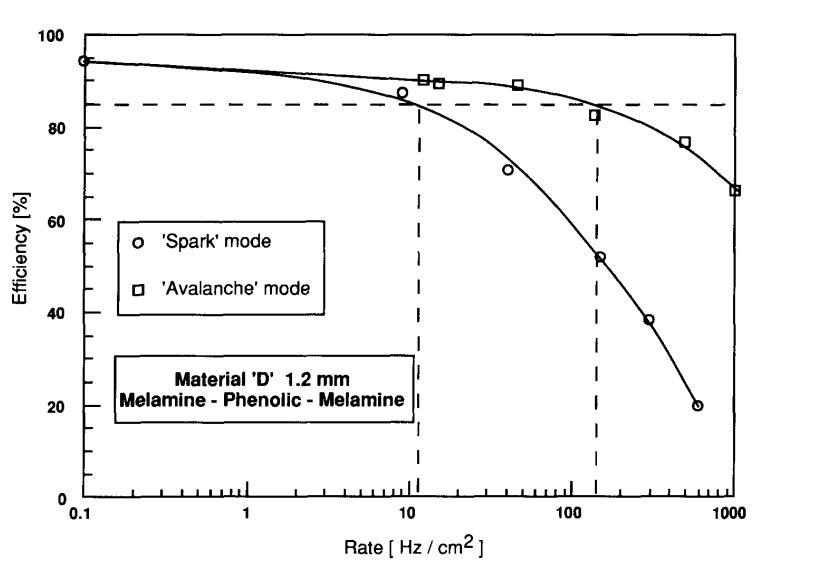
\includegraphics[width = \plotwidth]{fig/chapt4/Rate_Mode_Comparison.png}
		\caption{\label{fig:ModeRate} Rate capability comparison for the streamer and avalanche mode of operation. An order of magnitude in rate capability for a maximal efficiency drop of 10\% is gained by using the avalanche mode over the streamer mode.}
	\end{figure}

	\subsection{Standard gas mixture for RPCs operated in collider experiments}
	\label{chat4:ssec:gasmix}
	
	The first RPC working in streamer mode was operated with a 50/50 mixture of argon and butane~\cite{SANTONICO81}, a standard mixture used at that time in multi-wire proportional chambers, taking profit of the good effective Townsend coefficient of argon to maximize the number of primary charge carriers freed in the gas by ionizing particles and of the quenching properties of butane. Before the discovery of the avalanche mode of RPC operation and concerned about the rate capability of RPCs operated in streamer mode, the performance improvement of the detectors through the increase of fast charge proportion in the signal development was studied by adding Freon based gases, such as $CF_3Br$~\cite{CARDARELLI93}, into the typical $Ar$/$C_4H_{10}$ gas mixture.
	
	The typical gas mixture RPCs are operated with is generally composed of the following 3 gas compounds, although, as mentioned in Chapter~\ref{chapt3:sec:EcoGas}, research is being conducted into new more ecofriendly gas mixture using gases with a much lower \acl{GWP}:
	
	\begin{itemize}
		\item[•] Tetrafluoroethane ($C_2F_4H_2$), also referred to as \textit{Freon} or \textit{R134a}, is the principal compound of the RPC gas mixtures, with a typical fraction above 90\%. It is used for it's high effective Townsend coefficient and the great average fast charge that allows to operate the detector with a high threshold with respect to argon, for example, that has similar effective Townsend coefficient but suffers from a lower fast charge. To operate with similar conditions, argon would require a higher electric field leading to a higher fraction of streamers, thus limiting the rate capability of the detector~\cite{ABBRESCIA1997}.
		\item[•] Isobutane (i-$C_4H_{10}$), only present in a few percent in the gas mixtures, is used for its UV quenching properties~\cite{BATTISTONI85} helping to prevent streamers due to UV photon emission during the avalanche growth.
		\item[•] Sulfur hexafluoride, ($SF_6$), simply referred to as \textit{SF6}, is used in very little quantities for its high electronegativity. Excess of electrons are being absorbed by the compound and streamers are suppressed~\cite{ZEBALLOS98}. Nevertheless, a fraction of $SF_6$ higher than 1\% will not bring any extra benefice in terms of streamer cancelation power but will lead to higher operating voltage~\cite{CAMARRI98}, as can be understood through Figure~\ref{fig:SF6}.
	\end{itemize}
	
	\begin{figure}[H]
		\centering
		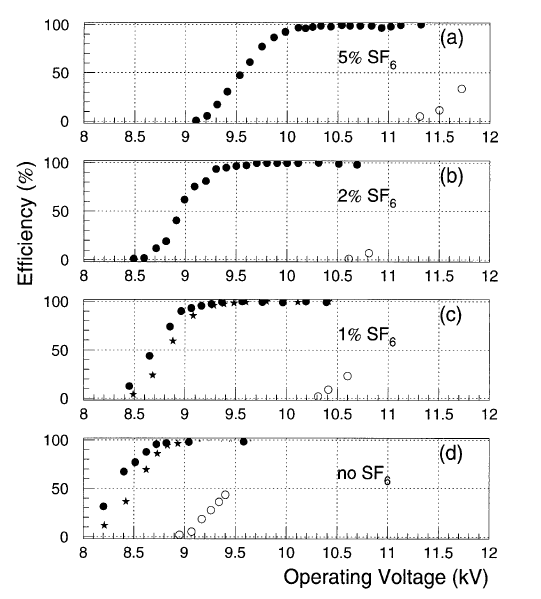
\includegraphics[width = 0.7\plotwidth]{fig/chapt4/SF6.png}
		\caption{\label{fig:SF6} Effeciency (circles and stars with \SI{30}{mV} and \SI{100}{mV} thresholds respectively) and streamer probability (opened circles) as function of the operating voltatge of a \SI{2}{mm} single gap HPL RPC flushed with a gas mixture containing (a) 5\%, (b) 2\%, (c) 1\% and (d) no $SF_6$~\cite{CAMARRI98}.}
	\end{figure}
	
	\subsection{Electron drift velocity}
	\label{chapt4:ssec:drift}
	
	{\color{blue} Talk about the electron drift velocity and mention the time resolution of RPCs.}
	
	\subsection{Detector designs and performance}
	\label{chapt4:ssec:design}
	
	Different RPC design have been used and each of them present its own advantages. Historically, the first type of RPC to have been developed is what is referred now to \textit{noarrow gap} RPC~\cite{SANTONICO81,ZEBALLOS96COMP}. After the avalanche mode has been discovered~\cite{CROTTY93}, it has been proven that increasing the width of the gas gap lead to higher rate capability, due to lower charge deposition per avalanche, and lower power dissipation~\cite{ZEBALLOS96COMP}. Nevertheless, by increasing the gas gap width, the time resolution of the detector decreases. This is a natural result if the increase of active gas volume in the detector is taken into account. Indeed, for a given threshold, only the small fraction of gas closest to the cathode will provide enough gain to have a detectable signal. In the case of a wider gas volume, the active region is then larger and a larger time jitter is introduced with the variation of starting position of the avalanche, as discussed in~\cite{ZEBALLOS96MRPC}. To solve improve both the time resolution and the rate capability, different methods were used trying to get advantages of both narrow and wide gap RPCs.
	
		\subsubsection{Double-gap RPC}
		\label{chapt4:sssec:DGRPC}
	
	Double-gap RPCs are made out of 2 narrow RPC detectors. The 2 RPC gaps are stacked on top of each other as shown in Figure~\ref{fig:DGLayout}. This detector layout, popularized by the two multipurpose experiments CMS~\cite{MUONTDR} and ATLAS~\cite{ATLASTDR} at LHC, can be used as an OR system in which each individual chamber participates in the ouput signal. The gain of such a detector is greatly reduced with respect to single-gap RPCs with an efficiency plateau reached at lower voltage, as visible on Figure~\ref{fig:DoubleGap}.
	
	\begin{figure}[H]
		\centering
		\includegraphics[width = \plotwidth]{fig/chapt4/Double_gap_layouts.pdf}
		\caption{\label{fig:DGLayout} Possible double-gap RPC layouts: a) "standard" 1D double-gap RPC, as used in CMS experiment, where the anodes are facing each other and a 1D read-out plane is sandwished in between them,  b) double read-out double-gap RPC as used in ATLAS experiment, where the cathodes are facing each other and 2 read-out planes are used on the outter surfaces. This last layout can offer the possibility to use a 2D reconstruction by using orthogonal read-out planes.}
	\end{figure}
	
	\begin{figure}[H]
		\begin{subfigure}{0.5\linewidth}
			\centering
			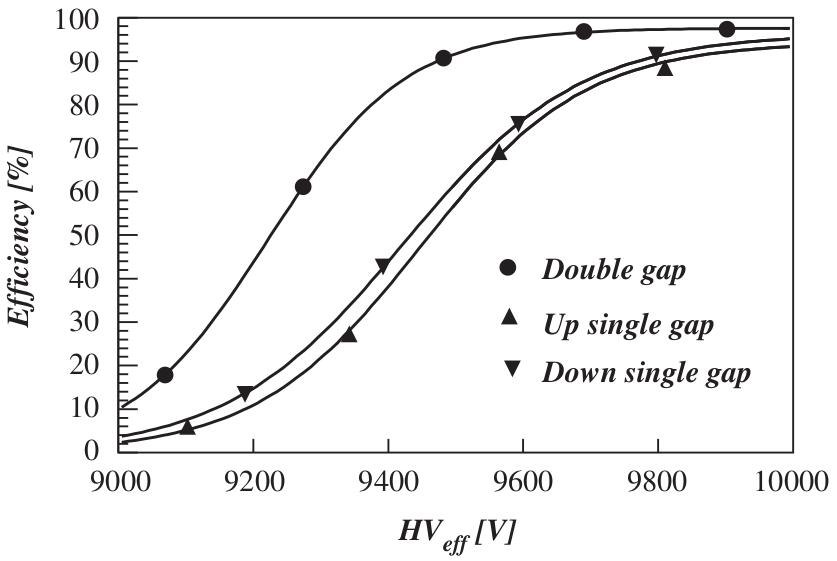
\includegraphics[width = 0.5\plotwidth]{fig/chapt4/Double-gap-Sigmoid.png}\\
			\caption{\label{fig:DoubleGap:A}}
		\end{subfigure}
		\begin{subfigure}{0.5\linewidth}
			\centering
			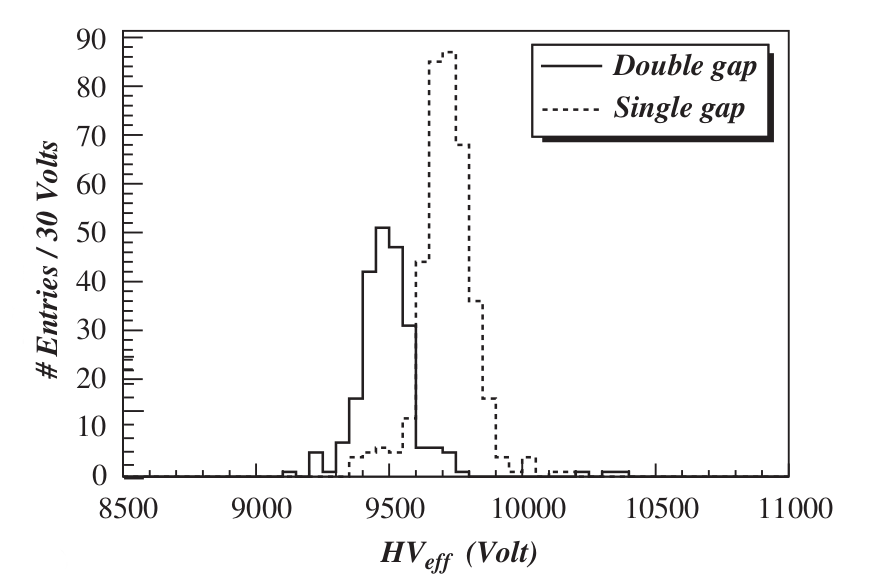
\includegraphics[width = 0.5\plotwidth]{fig/chapt4/Double-gap-Eff-95.png}
			\caption{\label{fig:DoubleGap:B}}
		\end{subfigure}
		\begin{subfigure}{\linewidth}
			\centering
			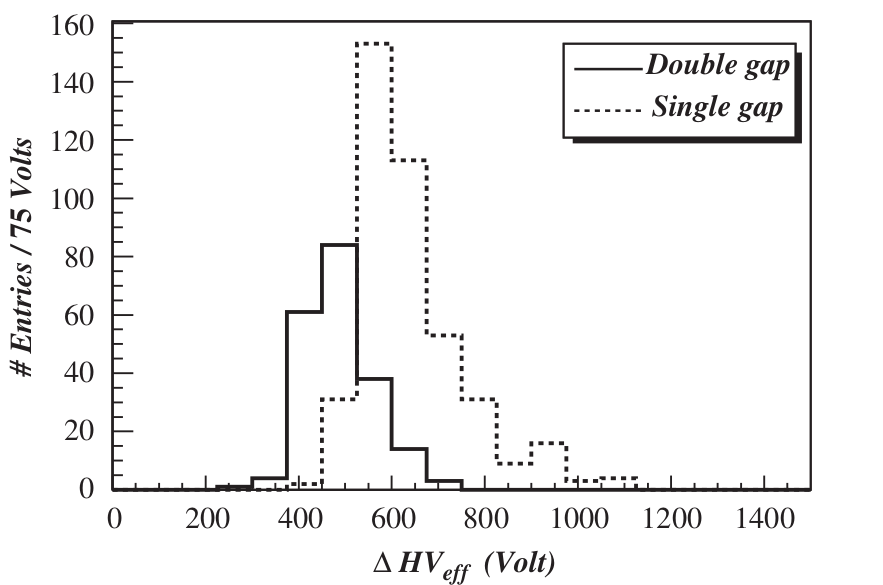
\includegraphics[width = 0.5\plotwidth]{fig/chapt4/Double-gap-Eff-Delta-90-10.png}
			\caption{\label{fig:DoubleGap:C}}
		\end{subfigure}
		\caption{\label{fig:DoubleGap} Comparison of performance of CMS double and single gap RPCs using cosmic muons~\cite{ABBRESCIA2005}. Figure~\ref{fig:DoubleGap:A}: Comparison of efficiency sigmoids. Figure~\ref{fig:DoubleGap:B}: Voltage distribution at 95\% of maximum efficiency. Figure~\ref{fig:DoubleGap:C}: $\Delta^{90\%}_{10\%}$ distribution.}
	\end{figure}
	
		\subsubsection{Multigap RPC (MRPC)}
		\label{chapt4:sssec:MRPC}
	
	MRPCs are layouts in which floating sub electrode plates are placed into a wide gap RPC to divide the gas volume and create a sum of narrow gaps~\cite{ZEBALLOS96MRPC,WILLIAMS98}. The time resolution of such a detector can reach of few tens of \si{ps}, with gas gaps of the order of a a few hundred \si{\micro m} as shown in Figure~\ref{fig:MRPC} representing ALICE \acf{ToF} MRPCs.
	
	\begin{figure}[H]
		\centering
		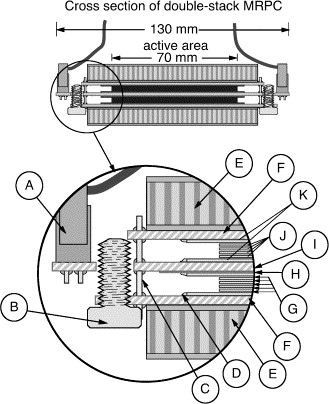
\includegraphics[width = 0.6\plotwidth]{fig/chapt4/MRPC-Layout.png}\\
		\caption{\label{fig:MRPC} Presentation of ALICE MRPC using \SI{250}{\micro m} gas gaps, \SI{620}{\micro m} outer glass electrodes and \SI{550}{\micro m} inner floating electrodes. More details on the labels are given in~\cite{ALICE2002}.}
	\end{figure}
	
	Sometimes used as a double multigap RPC, taking advantage of the OR of double gap RPCs, the MRPC is mainly used as ToF detector~\cite{ALICE2002,START2002,BESIII2014,CBM2007,MPD2016} due to it's excellent timing properties that allow to perform particle identification as explained by Williams in~\cite{WILLIAMS2012}. The principle of particle identification using ToF is simply the measurement of the velocity of a particle. Indeed, particles are defined by their mass (for the parameter of interest here, their electric charge being measured using the bending angle of the particles traveling through a magnetic field) and this mass can be calculated by measuring the velocity $\beta$ and momentum of the particle:
	
	\begin{equation}
		\beta = \frac{p}{\sqrt{p^2 + m^2}}
	\end{equation}
	
	Intuitively, it is trivial to understand that 2 different particles having the same momentum will have a different velocity due to the mass difference and thus a different flight time $T_1$ and $T_2$ through the detector and this is used to separate and identify particles. The better the time resolution of the ToF system used, the stronger will the separation be:
	
	\begin{equation}
		T = \frac{L}{v} = \frac{L}{c\cdot\beta}, \quad \Delta T = T_1 - T_2 = \frac{L}{c}\left(\sqrt{1+m_1^2/p^2} - \sqrt{1+m_2^2/p^2}\right) \cong (m_1^2 - m_2^2)\frac{L}{2cp^2}
	\end{equation}
	
	An example of particle identification is given for the case of STAR experiment in Figure~\ref{fig:ParticleID}.
	
	\begin{figure}[H]
		\centering
		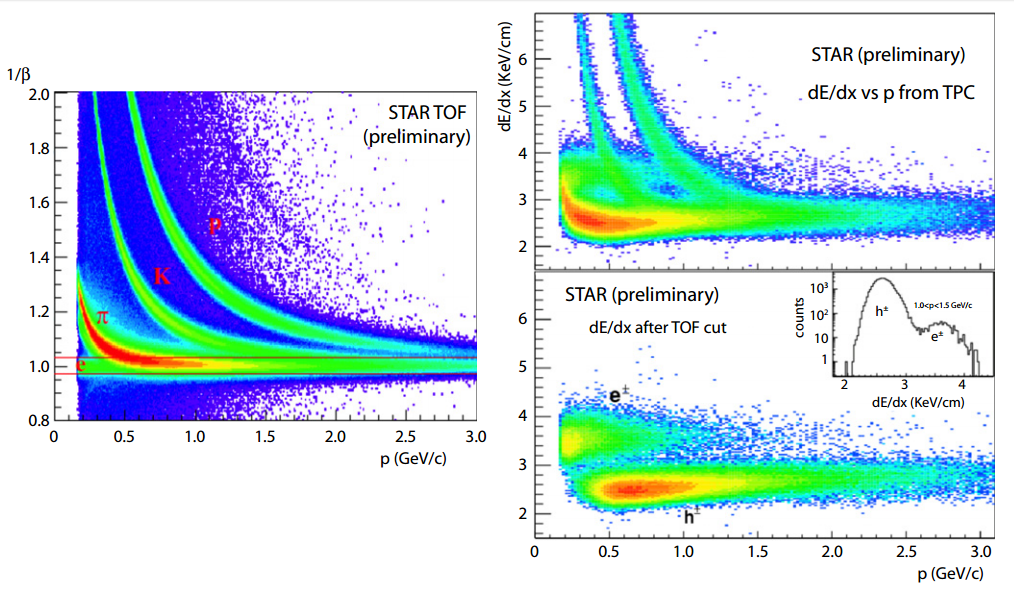
\includegraphics[width = \plotwidth]{fig/chapt4/STAR-ToF.png}\\
		\caption{\label{fig:ParticleID} Particle identification applied to electrons in the STAR experiment. The identification is performed combining ToF and $dE/dx$ measurements~\cite{WILLIAMS2012}.}
	\end{figure}
	
	Another benefice of using such small gas gaps is the strong reduction of the average avalanche volume and thus of the blind spot on MRPCs leading to an improved rate capability. Multigaps can sustain backgrounds of several \si{kHz/cm^2} as demonstrated in Figure~\ref{fig:MRPCRate}.
	
	\begin{figure}[H]
		\centering
		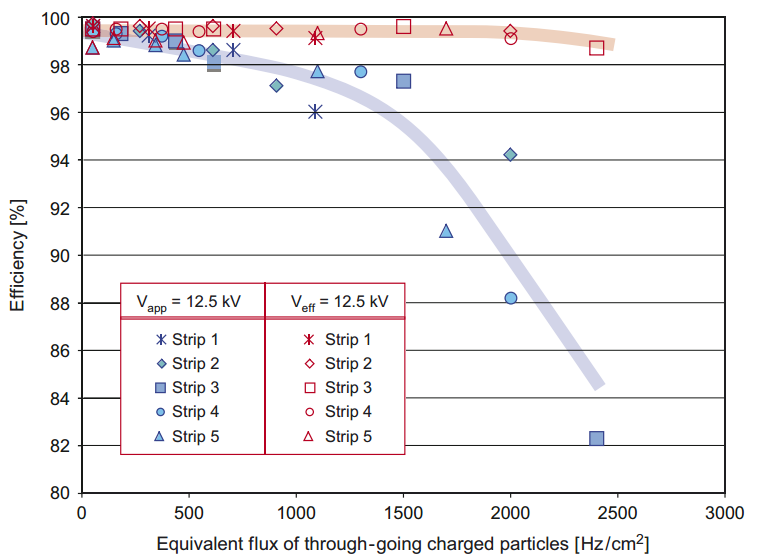
\includegraphics[width = 0.7\plotwidth]{fig/chapt4/ALICE-Rate_Capability.png}\\
		\caption{\label{fig:MRPCRate} Comparison of the detector performance of ALICE ToF MRPC~\cite{ALICI2007} at fixed applied voltage (in blue) and at fixed effective voltage (in red). The effective voltage is kept fixed by increasing the applied voltage accordingly to the current drawn by the detector.}
	\end{figure}
	
		\subsubsection{Charge distribution and performance limitations}
		\label{chapt4:sssec:charge}
		
	The direct consequence of the different RPC layouts is a variation of intrinsic time resolution of the RPC as the gap size decreases. An advantage is given to multigaps whose design use sub-millimeter gas volumes providing very consistent signals.
	
	On the charge spectrum point of view, each layout has its own advantages. When the double-gap has the highest induced over drifting charge ratio, as seen in Figure~\ref{fig:ChargeRatio}, the multigap has a charge spectrum strongly detached from the origin, as visible in Figure~\ref{fig:ChargeSpectra}. A high induced over drifting charge ratio means that the double gap can be safely operated at high threshold or that at similar threshold it can be operated with a twice smaller drifting charge, meaning a higher rate capability. On the other hand, the strong detachment of the charge spectrum from the origin in the MRPC case allows to reach a higher efficiency with increasing threshold as most of the induced charge is not low due to the convolution of several single gap spectra. The range of stable efficiency increases with the number of gap, as presented in Figure~\ref{fig:EffThreshold}.
	
	\begin{figure}[H]
		\centering
		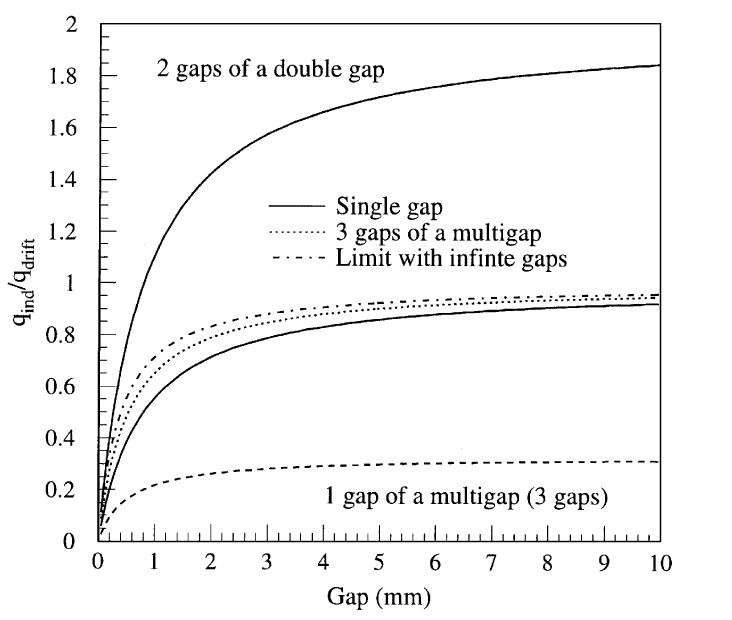
\includegraphics[width = 0.6\plotwidth]{fig/chapt4/Layout_charge_ratio.png}\\
		\caption{\label{fig:ChargeRatio} Ratio between total induced and drifting charge have been simulated for single gap, double-gap and multigap layouts~\cite{ABBRESCIA99}. The total induced charge for a double-gap RPC is a factor 2 higher than for a multigap.}
	\end{figure}
	
	\begin{figure}[H]
		\centering
		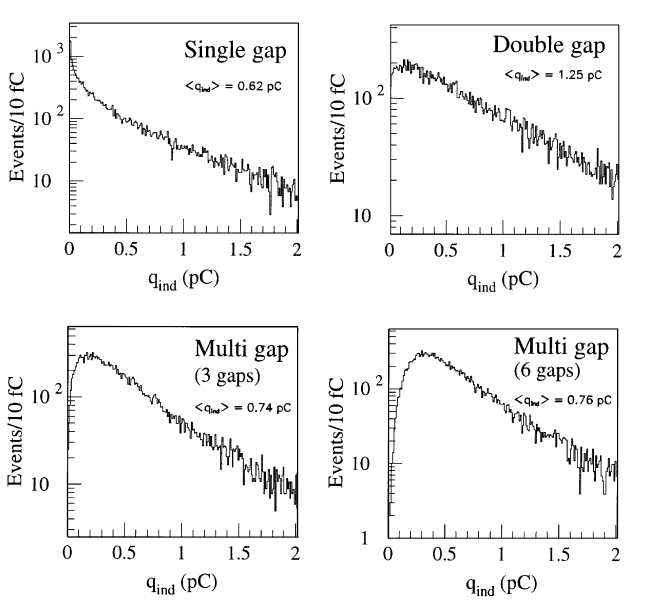
\includegraphics[width = \plotwidth]{fig/chapt4/Layout_charge_distributions.png}\\
		\caption{\label{fig:ChargeSpectra} Charge spectra have been simulated for single gap, double-gap and multigap layouts~\cite{ABBRESCIA99}. It appears that when single gap shows a decreasing spectrum, double and multigap layouts exhibit a spectrum whose peak is detached from the origin. The detachment gets stronger as the number of gaps increases.}
	\end{figure}
	
	\begin{figure}[H]
		\centering
		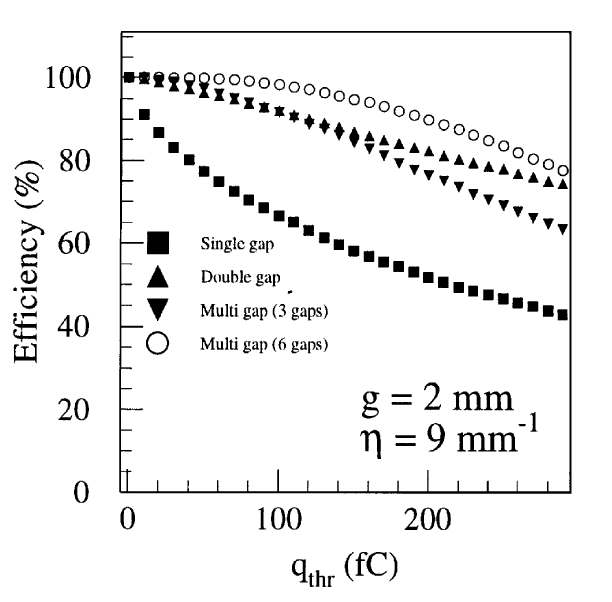
\includegraphics[width = 0.6\plotwidth]{fig/chapt4/Layout_eff_vs_thr.png}\\
		\caption{\label{fig:EffThreshold} The maximal theoretical efficiency is simulated for single gap, double-gap and multigap layouts~\cite{ABBRESCIA99} at a constant gap thickness of \SI{2}{mm} and using an effective Townsend coefficient of \SI{9}{mm^{-1}}.}
	\end{figure}

\section{Signal formation}
\label{chapt4:sec:signal}

\section{Gas transport parameters}
\label{chapt4:sec:transport}



\clearpage{\pagestyle{empty}\cleardoublepage}
